\documentclass[tikz,border=10pt]{standalone}
% Shared look for every TikZ diagram. Load with \input{../../tools/tikz-style.tex}
\usepackage[T1]{fontenc}
\usepackage{lmodern}
\renewcommand{\sfdefault}{lmr}  % diagrams use the same serif as the text
\usetikzlibrary{arrows.meta, positioning, shapes.geometric, calc, fit, backgrounds}
\definecolor{cblue}{HTML}{4C78A8}
\definecolor{corange}{HTML}{F58518}
\definecolor{cgreen}{HTML}{54A24B}
\definecolor{cred}{HTML}{E45756}
\definecolor{cpurple}{HTML}{B279A2}
\definecolor{cgrey}{HTML}{6B6B6B}
\tikzset{
  every picture/.style={font=\sffamily, line width=1.2pt},
  box/.style={draw=#1, fill=#1!12, rounded corners=4pt, align=center, inner sep=7pt, minimum height=1.1cm},
  box/.default=cgrey,
  arrow/.style={-{Stealth[length=3mm]}, draw=cgrey, line width=1.4pt},
  title/.style={font=\sffamily\bfseries\Large},
  note/.style={font=\sffamily\small, text=cgrey, align=center},
}
\AtBeginDocument{\hyphenpenalty=10000 \exhyphenpenalty=10000}

\begin{document}
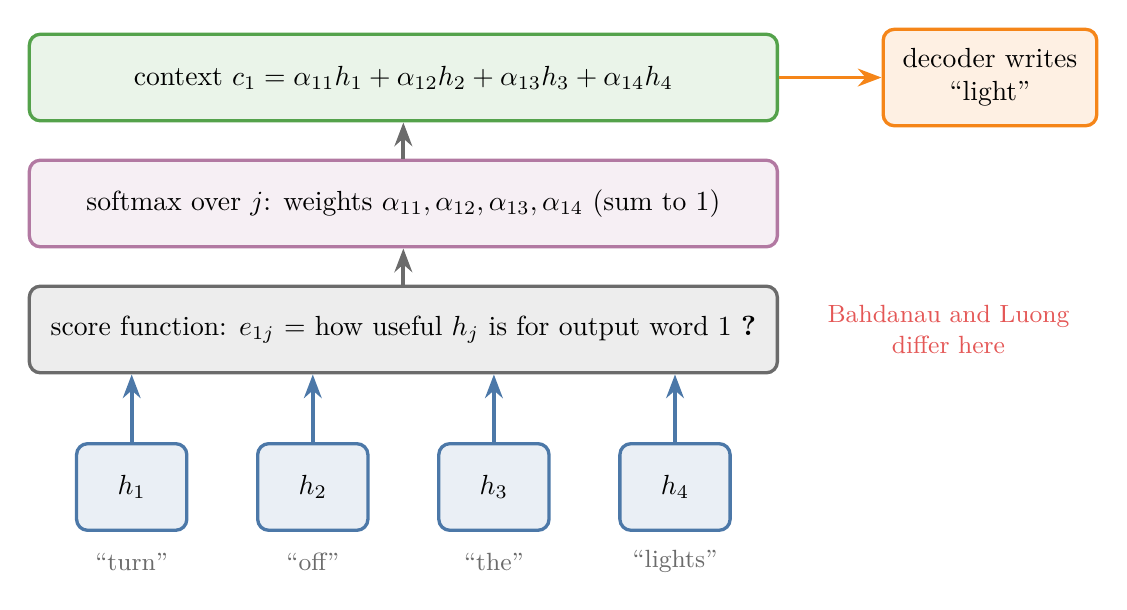
\begin{tikzpicture}[h/.style={box=cblue, minimum width=1.4cm, font=\sffamily}]
  \foreach \w [count=\j] in {turn, off, the, lights} {
    \node[h] (h\j) at (2.3*\j,0) {$h_\j$};
    \node[note] at (2.3*\j,-0.95) {``\w''};
  }
  \node[box=cgrey, minimum width=9.5cm] (sc) at (5.75,2.0) {score function: $e_{1j}$ = how useful $h_j$ is for output word 1 \textbf{?}};
  \foreach \j in {1,...,4} \draw[arrow, draw=cblue] (h\j) -- (h\j |- sc.south);
  \node[box=cpurple, minimum width=9.5cm] (sm) at (5.75,3.6) {softmax over $j$: weights $\alpha_{11}, \alpha_{12}, \alpha_{13}, \alpha_{14}$ (sum to 1)};
  \draw[arrow] (sc) -- (sm);
  \node[box=cgreen, minimum width=9.5cm] (c) at (5.75,5.2) {context $c_1 = \alpha_{11} h_1 + \alpha_{12} h_2 + \alpha_{13} h_3 + \alpha_{14} h_4$};
  \draw[arrow] (sm) -- (c);
  \node[box=corange] (d) at (13.2,5.2) {decoder writes\\``light''};
  \draw[arrow, draw=corange] (c) -- (d);
  \node[note, text=cred, anchor=west] at (11.0,2.0) {Bahdanau and Luong\\differ here};
\end{tikzpicture}
\end{document}
